%!TEX root = thesis.tex

\chapter{Body Part Detection}
\label{ch:bodyparts}

To perform hand pose estimation of a person in a image, hands need to be localized in the image first. Hands are very deformable - they can have very different appearances and different orientations. Also hand size, hand shape and skin color can differ tremendously per person. This makes localization a  difficult task. 

One way to localize the hands is by searching for skin like colors in an image given a pre-calculated color profile. A generic skin color model based on average skin color has been constructed for this purpose\cite{Jones1999}. The problem with this method is that it fails when the skin color isn't 'pure', for example when it is colored by a light source. Also, since the profile is very generic, it contains colors for many different skin colors. This introduces more false positives.

It would be much better to have a method for obtaining the skin color of a person in a image from that image itself. This can be done by extracting the skin model from the face, which is much easier to detect.

This chapter describes how a skin model is created and how this is used to find the skin pixels in the image. These found skin pixels are clustered and labeled as left hand, right hand and head. 

\section{Skin Segmentation}
\label{sec:skinmodel}

\subsection*{Face localization}

\begin{figure}
  \center{}
    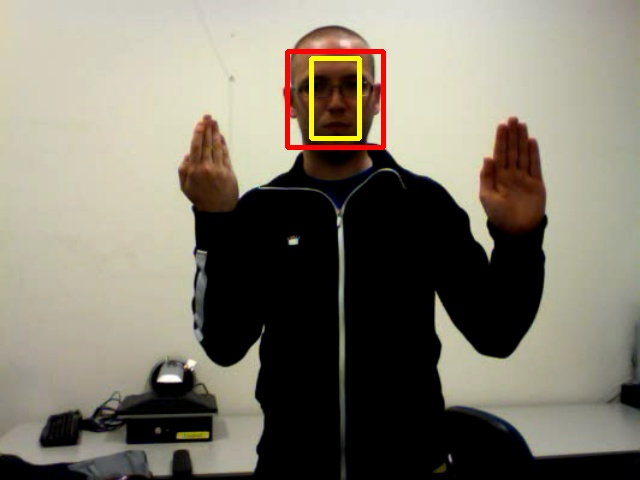
\includegraphics[width=0.6\textwidth]{figures/pipeline/detected.jpg}
  \caption{Face detection}
  \label{fig:face_detection}
\end{figure}

Finding faces in a image is a rather well solved problem. A face is easy to detect, since it is almost non-deformable. Different faces are quite similar looking at the most prominent properties. People don't tilt their head often or not more than a couple degrees, which makes it even more easier to detect. Face detection can be done in a fast and robust way using a haar classifier, a boosted rejection cascade that is trained with Haar\-like wavelet\cite{Lienhart2002}. This is a method for detecting faces that doesn't rely on color information. The classifier is run over the image on different scales, and positions with a score above a certain threshold are classified as face position, see \autoref{fig:face_detection} for an example. In the figure you can see the complete head and surrounding (yellow rectangle) is returned by the search algorithm. Since we are only interested in the skin pixels a smaller sub-region is used for further processing.

Still, the face detection is a expensive operation. Fortunately a face doesn't move fast in a vide stream, a number of frames can be skipped which will free more computational time for other operations.

Using a classifier to search for a face and obtain a skin color profile from it has been done before with the lab color space \cite{Stenger2006}, but in this case the HSV color space is used.



\subsection*{Color Space Conversion}
Usually, pixel values of a image are stored in the Red, Green Blue (RGB) color space where colors are represented with combinations of these primary colors. The RGB representation of colors is not suitable for modeling skin color. The RGB color space represents not only color, but also luminance which is not a reliable measure for segmenting skin pixels\cite{Cai1999}.

When a subject is lighted by a light source with uniform hue distribution, the light doesn't change the hue or saturation of the subject. The only thing that will change is the luminance, which is changing because of the light source's intensity, distance or (self casted) shadow. Since we want to extract hand pixels independent of the illumination intensity, we can ignore this channel and only use the hue and saturation.

The luminance can be removed from the color space by transforming the color model to a chromatic color space. There are multiple chromatic color spaces\cite{Bradski1998}, for example LAB, HSV and normalized RGB. A small experiment with these color spaces have shown that no significant improvements can be gained with a specific color space, so the HSV color space is used in the rest of this paper.

\begin{figure}[htbp]
  \centering
\subfloat[HSV color space]{
	\label{fig:hsv}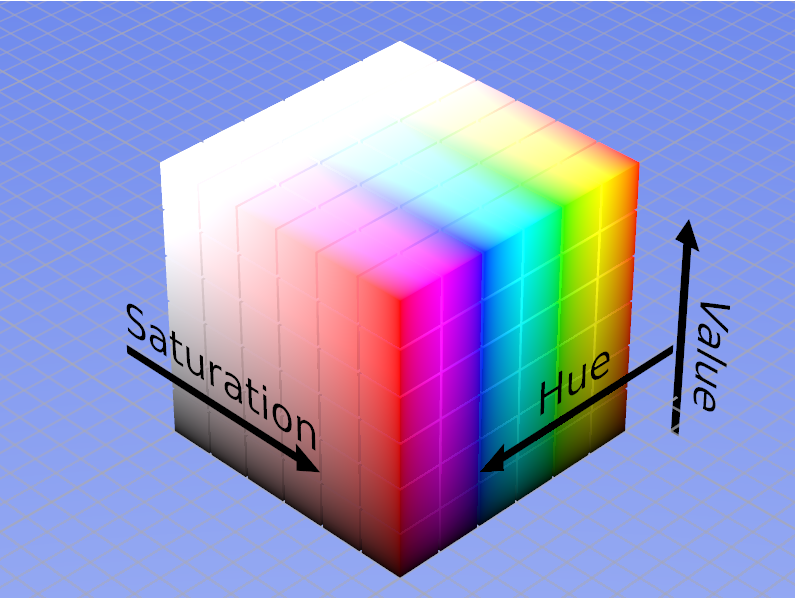
\includegraphics[width=0.45\linewidth]{figures/hsv2.png}
}
\hspace{0.01\linewidth}
\subfloat[RGB color space]{
	\label{fig:rgb}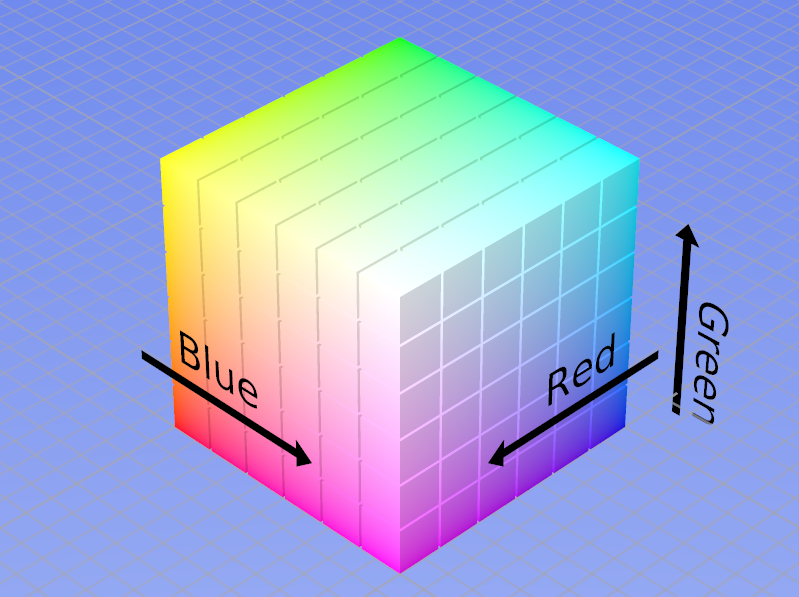
\includegraphics[width=0.45\linewidth]{figures/rgb.png}
}
  \caption{The RGB and HSV color space}
  \label{fig:colorspaces}
\end{figure}

HSV stands for hue (color), saturation (how concentrated the color is) and value (brightness). In practice a light source never has a uniform distribution and \emph{will} change the color of the subject. Since we build a color model from the image itself, all skin pixels will change in the same way. 

The RGB color space is transformed into the HSV color space using the following equations:


\begin{eqnarray}
  V & \leftarrow & \max(R,G,B) \\
  S & \leftarrow & \left\{
  \begin{array}{l l}
    \frac{V-\min(R, G, B)}{V} & \quad \text{if $V \neq 0$} \\
    0 						  & \quad \text{otherwise} \\
  \end{array} \right.\\
  H & \leftarrow & \left\{
  \begin{array}{l l}
    \frac{60(G - B)}{S}     & \quad \text{if $V = R$} \\
    \frac{120 + 60(B-R)}{S} & \quad \text{if $V = G$} \\
    \frac{240 + 60(R-G)}{S} & \quad \text{if $V = B$} \\
  \end{array} \right.
\end{eqnarray}

Note that for computation simplicity this a simplification of the real HSV color space. The real HSV colorspace is circular in the Hue dimension.

The input 3 channel RGB image is transformed into a 3 channel HSV image, after which the value channel is discarded. Using the detected face region of the hue and saturation channel a histogram can be constructed which will represent a statistical skin model.

\begin{figure}[htbp]
  \centering
\subfloat[hue channel]{\label{fig:hue}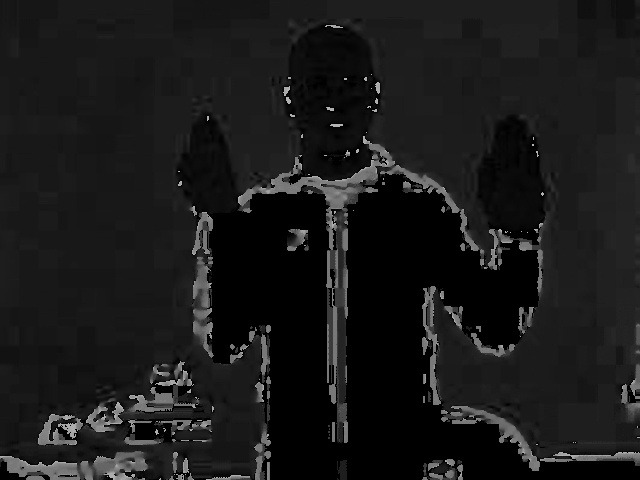
\includegraphics[width=0.3\linewidth]{figures/pipeline/hue.jpg}}
\hspace{0.03\linewidth}
\subfloat[saturation channel]{\label{fig:saturation}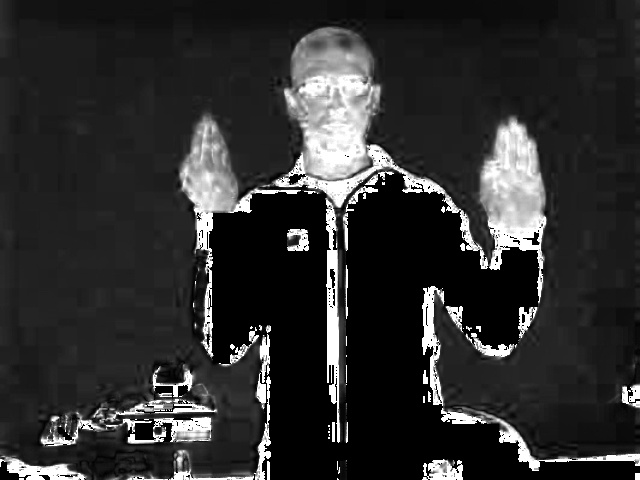
\includegraphics[width=0.3\linewidth]{figures/pipeline/saturation.jpg}}
\hspace{0.03\linewidth}
\subfloat[value channel]{\label{fig:value}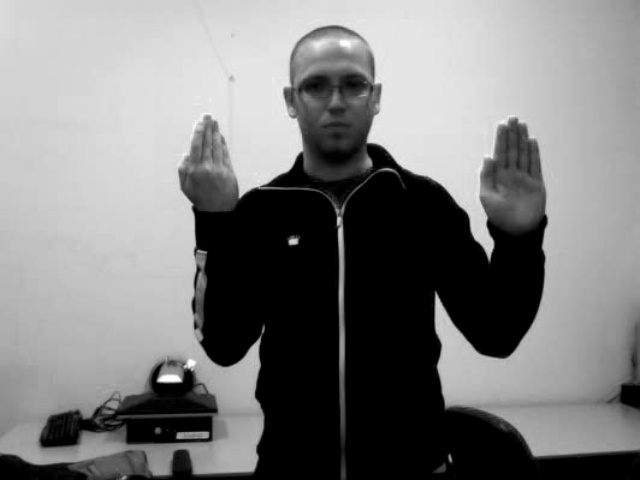
\includegraphics[width=0.3\linewidth]{figures/pipeline/value.jpg}}
  \caption{The HSV channels}
  \label{fig:hsvchannels}
\end{figure}





\subsection*{Statistical Skin Color Model}

\begin{figure}[htbp]
    \center{}
    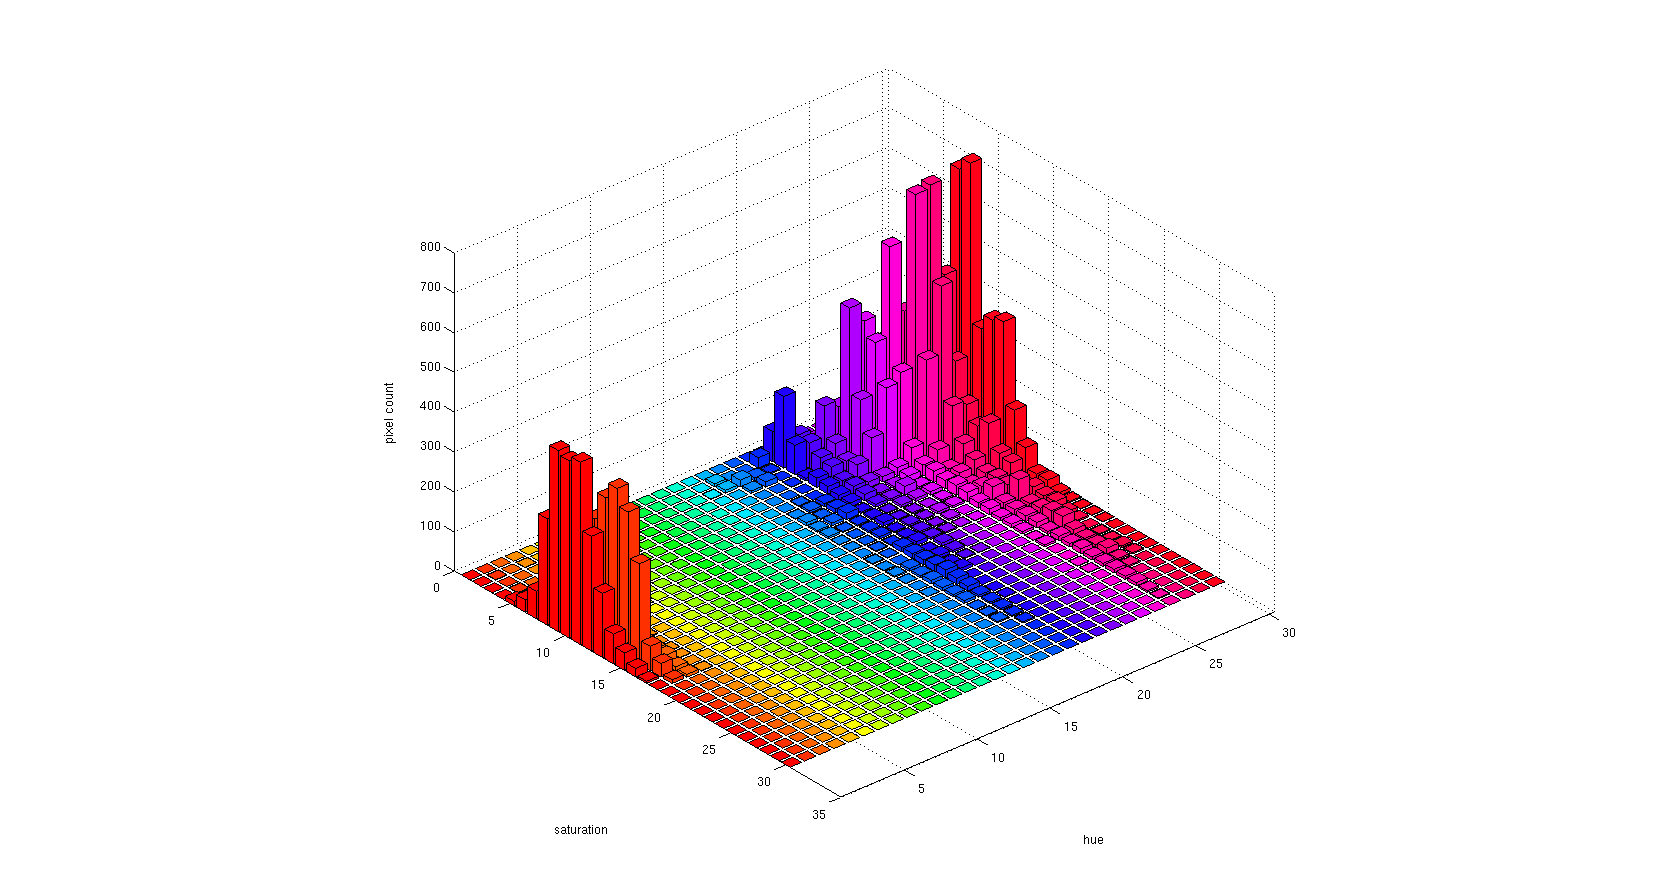
\includegraphics[width=1\textwidth]{figures/pipeline/histogram.png}
	\caption{A histogram of face pixels}
	\label{fig:histogram}
\end{figure}

There are multiple ways of constructing a statistical skin color model. The most conventional ways are a (mixture of) gausian(s) or a histogram. 

The skin color model is represented in a 2 dimensional histogram, where the first dimension is Hue and the second is Saturation. The histogram is filled with the values from the detected face region. After, the histogram is normalized - all values are divided by the sum of all bins. This makes the histogram independent of the original image size, and each histogram bin value represents a 'skin probablility'. \autoref{fig:histogram} is a histogram of colors of a caucasian.

Manual experiments show that tweaking the number of bins doesn't have much effect, as long as the number of bins is not too high or not to low. Since for the storage of the values a 8 bit integer is used, a number of bins higher than 256 doesn't make sense. In all experiments mentioned in this paper a number of bins of 30 is used for both the hue and saturation.

\subsection*{Back Projection}

\begin{figure}[htbp]
    \center{}
    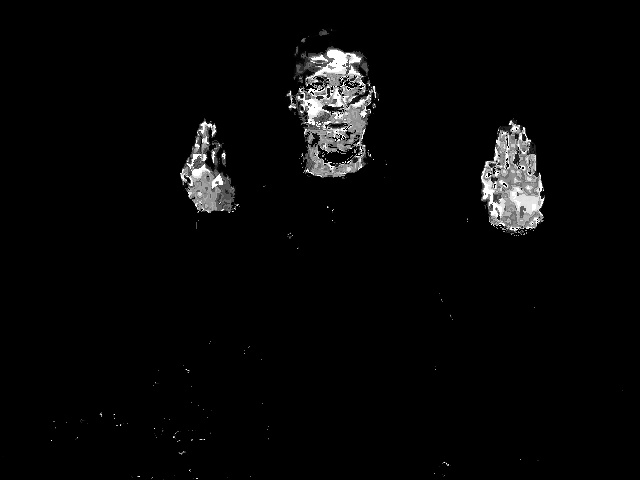
\includegraphics[width=0.5\textwidth]{figures/pipeline/backproject.jpg}
 	\caption{Backprojection}
	\label{fig:backproject}
\end{figure}


A back projection is the combination of an image and a histogram. The result is a new single channel image. All pixels in the input image are iterated and the corresponding bins are looked up in the histogram. The pixel in the same position in the new image is replaced with the value from the histogram. If the histogram is a skin color histogram, the resulting image will have high values for pixels that are skin-like pixels, and low values for other pixels. The result of the process can be seen in \autoref{fig:backproject}. Since the probabilities are very low the contrast of this image is enhanced so the maximum pixel value becomes pure white.


\subsection*{Smoothing}
The back projection can be quite noisy, this is caused by the rounding in the in the histogram, but also by noise introduced by the camera. Thresholding this image will result in skin pixel groups with rough edges and a lot of holes, see \autoref{fig:threshold_noblur}. The noise can be reduced by smoothing the image. This way, the pixel value is replaced by the old value weighted with the surrounding pixel values. Using a gaussian kernel with a large size gives a good result, see \autoref{fig:blurred}.

\begin{figure}[htbp]
    \center{}
    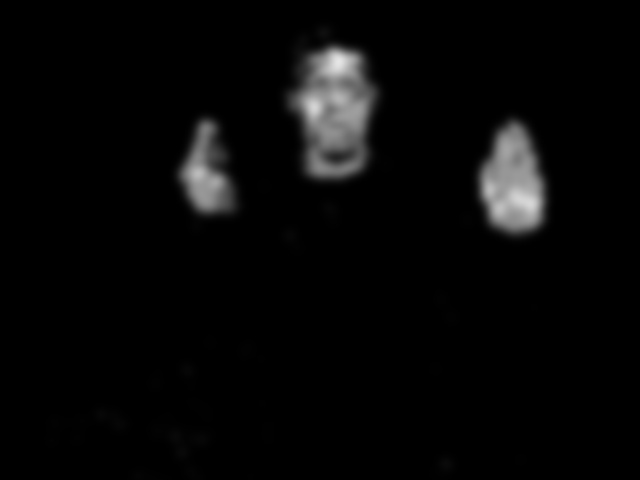
\includegraphics[width=0.5\textwidth]{figures/pipeline/blurred.jpg}
	\caption{Blurred image}
	\label{fig:blurred}
\end{figure}


\subsection*{Threshold}

\begin{figure}[htbp]
    \center{}
 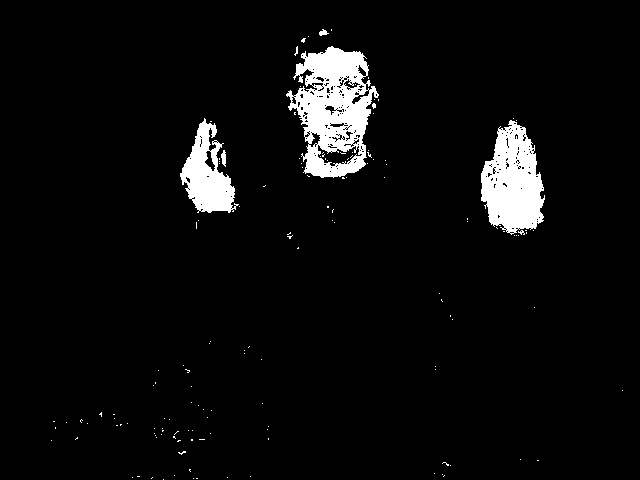
\includegraphics[width=0.5\textwidth]{figures/pipeline/thresholded_noblur.jpg}
	\caption{Thresholded image without blur preprocessing}
	\label{fig:threshold_noblur}
\end{figure}

\begin{figure}[htbp]
    \center{}
    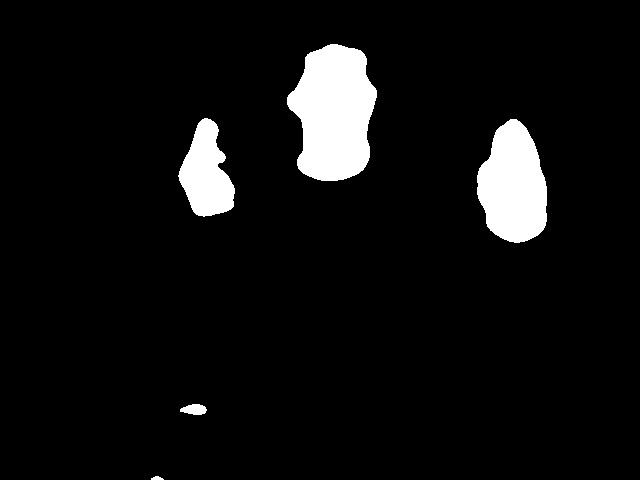
\includegraphics[width=0.5\textwidth]{figures/pipeline/thresholded.jpg}
	\caption{Thresholded image}
	\label{fig:threshold}
\end{figure}


To segments pixels from non-skin pixels we need to define a way of doing this automatically. The easiest way to accomplish this is by defining a threshold. All pixel values below a certain threshold are replaced with false or 0, all above this threshold will be replaced with true or 1. This results in a binary image with labels for (non) skin pixels. This introduces one parameter - the 
threshold for going from the probabilistic domain to the binary domain.

A alternative method of going from the probabilistic domain to the binary domain is adaptive thresholding. here the threshold is determined per pixel by the values of surrounding pixels. This method has one parameter; the neighborhood blocksize used to determine the threshold.


\subsection*{Morphological Operations}

\begin{figure}[htbp]
    \center{}
    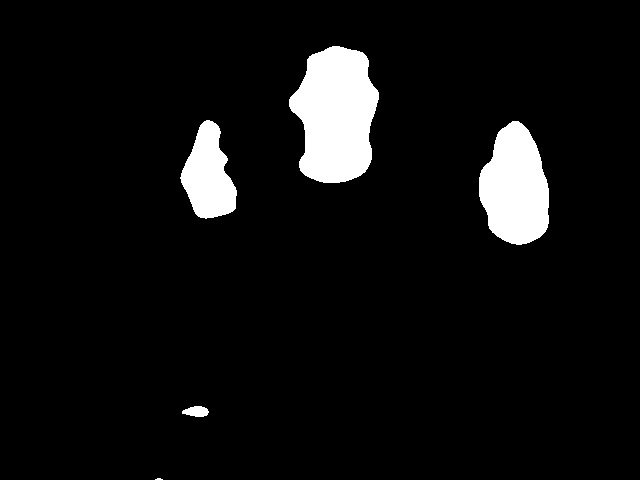
\includegraphics[width=0.5\textwidth]{figures/pipeline/closed.jpg}
	\caption{Morphologically closed}
	\label{fig:closed}
\end{figure}

An alternative to smoothing out rough edges and holes are (combinations of )morphological operations.  A morphologic closing operation of A by B is obtained by the dilation of A by B, followed by erosion of the resulting structure by B. The result of performing this operation is that small holes in the binary image are removed, and edges are smoothed as seen in \autoref{fig:closed}. The effect isn't really significant, since the gaussian smoothing already removes a lot of noise. 


\section{Object Localization}

\subsection*{Pixel Grouping, Contour Extraction}
To be able to say something useful about groups of pixels, one need to know which pixels belong together. This is done by clustering. In this case clustering is performed by grouping pixels together to touch horizontally and vertically. Each cluster of pixels is called a blob.

To handle the blobs in a time efficient way, it is good idea to extract the contours. This way interesting problems can be solved like if a certain pixel coordinate is inside a certain blob, the maximum or minimal horizontal or vertical position and hole removal.

Since it unusual to have holes in blobs that represent skin regions, these can be removed. This is done with the algorithm described in \cite{Suzuki1985}, where the contours of the blobs are extracted and all contours except the outer most contour are removed. This removes holes and islands in holes.

From the contours of the group a square region of interest is defined by calculating the outer borders of the group. This window is called the hand window from now on.

\subsection*{Blob Labeling}

\begin{figure}[htbp]
    \center{}
    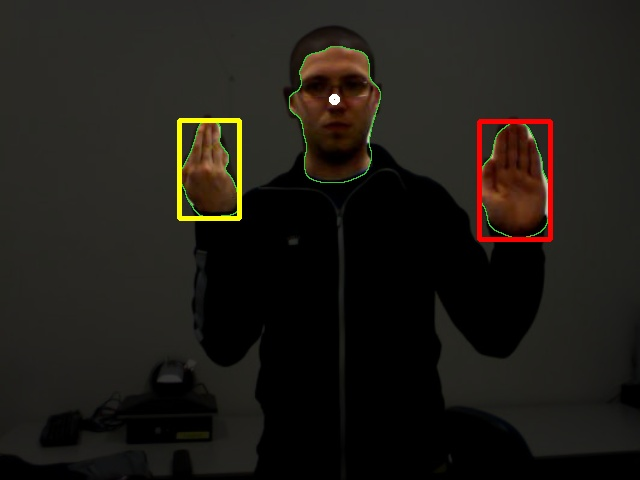
\includegraphics[width=0.5\textwidth]{figures/pipeline/contours.jpg}
	\caption{Labeled blobs}
	\label{fig:contours}
\end{figure}

(NEEDS REWRITE)

Now we have blobs we need to know blob is what body part. In a optimal situation there are three blobs, two for the hands and one for the head. For one blob it is already known what body part it is - the face. In the face detection phase we found a face in the image, so the blob containing the center point of the detected phase is the face blob. Usually the left hand is on the left of the head and the right hand on the right side. If there are three blobs, and the face is the middle blob, the labeling is finished. If not an other decision needs to be made. Often there are more or less blobs, because the background has skin-like color, a hand is difficult to detect or is occluded. Also the order of hands and head can change, a left hand doesn't necessarily need to appear on the left side of a head.

First the surface of each blob is calculated and then the blobs are sorted by size. The blob containing the head is removed from the list, since we already know this label. Also very small blobs are removed, because these are probably noise. The removal threshold surface is set to:

\begin{equation}
T = (\frac{h}{c})^2
\end{equation}

Where $h$ is the height of the movie frame and $c$ is a control constant. The equation can be interpreted as a filter for the minimal size in square pixels, relative to the hight of the movie frame. A value of $20$ for $c$ removes a lot of noise blobs, but still is small enough to leave most hand blobs intact.

Assuming the hands or the second biggest skin like objects in the image, the 2 or less biggest blobs are taken from the list and the rest is also discarded. If there is no biggest blob, the labeling is finished - there is only a head in the image. If there is one blob left, the left or right position relative to the head is the hand label. If there are 2 hands, there are 3 possible situations, 1 where the head is in the middle which is already described. If both hands are on the left of the head, the most outer left blob is labeled as left and the other as right. This is visa versa for right. This whole process is listed in \autoref{alg:blobheuristics}.

\begin{algorithm}
\caption{Blob labeling heuristics}
\label{alg:blobheuristics}
\begin{algorithmic}
   \REQUIRE A list of blobs 'blobs'
   \REQUIRE Coordinates of a face 'faceCenter'
   \ENSURE 3 or less blobs labeled head, left or right

	\FOR{blob in blobs}
		\IF{blob contains faceCenter}
			\STATE head $\leftarrow$ blob
			\STATE remove blob from blobs
		\ENDIF
	\ENDFOR

	\STATE keep only 2 biggest blobs
	\STATE sort blobs by $x$ position

	\STATE $n \leftarrow $ $|$blobs$|$
	\IF{$n = 2$}
	    \STATE left $\leftarrow$ blobs$_0$
	    \STATE right $\leftarrow$ blobs$_1$
	\ELSE
		\IF{$n = 1$}
		    \IF{center of blobs$_0$ $<$ center of face}
		        \STATE left $\leftarrow$ blobs$_0$
		    \ELSE
		        \STATE right $\leftarrow$ blobs$_0$
			\ENDIF
		\ENDIF
	\ELSE
	    \STATE no limbs found
	\ENDIF
\end{algorithmic}
\end{algorithm}



\subsection*{Blob label stabilization}
A hand doesn't move very fast in an image - usually it will not move from the left side to the right side in one frame. If this is detected this is probably a measurement error caused by noise or pour labeling. In this case the history of previous positions of a blob can be incorporated. This can be done with a Kalman Filter. A Kalman Filter is a easy and fast way of smoothing out the current position with the previous positions. The result will be a more stable estimation of the hand position. A second advantage of the Kalman Filter is the ability to actually predict the position of the hand in the next frame. This can become useful when there is no new hand detected. The hand position can then be estimated with a different method.

For every hand a Kalman filter is initialized. The measurement that need to be smoothed is the hand window. The hand window has a x and y position and a width and hight. Each hand also has a speed in the x and y direction but we don't measure that - we let the kalman filter represent, calculate and use that internally. 

A hand window represented in a measurement vector as:

\begin{equation}
 m_k = \left(
\begin{array}{c}
	x_k \\ %measurement.x
	y_k \\ %measurement.y,
	w_k \\ %measurement.width
	h_k \\ %measurement.height
\end{array} \right)
\end{equation}

Where $x_k$ is the horizontal position, $y_k$ is the vertical position, $w_k$ is the width and $h_k$ is the height of the hand window.

The Transition matrix is defined as follows:

\begin{equation}
 A = \left(
\begin{array}{cccccc}
	1 & 0 & 0 & 0 & 1 & 0 \\
	0 & 1 & 0 & 0 & 0 & 1 \\
	0 & 0 & 1 & 0 & 0 & 0 \\
	0 & 0 & 0 & 1 & 0 & 0 \\
	0 & 0 & 0 & 0 & 1 & 0 \\
	0 & 0 & 0 & 0 & 0 & 1 \\
\end{array} \right)
\end{equation}
	
This is just an identity matrix, except for the left ones on the right top in the matrix. These represent the combination of the current position and the internal state of the speed.

With these matrixes and a standard kalman filter the position and size of the hands can be predicted. The predicted values are used for an other hand localization method in case no hand is found en the next frame.

% setIdentity(kalman.measurementMatrix, Scalar(1));
% setIdentity(kalman.processNoiseCov, Scalar(1));
% setIdentity(kalman.measurementNoiseCov, Scalar(5));
% setIdentity(kalman.errorCovPost, Scalar(3));
% setIdentity(kalman.gain, Scalar(0e-15));
% randu(kalman.statePost, Scalar(1), Scalar(100));



% \paragraph{Update}
% The kalman filter is then updated:
% 
% Innovation or measurement residual 	
% $\tilde{\textbf{y}}_k = \textbf{z}_k - \textbf{H}_k\hat{\textbf{x}}_{k|k-1}$

% Innovation (or residual) covariance
% $\textbf{S}_k = \textbf{H}_k \textbf{P}_{k|k-1} \textbf{H}_k^\text{T} + % \textbf{R}_k$

% Optimal Kalman gain
% $\textbf{K}_k = \textbf{P}_{k|k-1}\textbf{H}_k^\text{T}\textbf{S}_k^{-1}$

% Updated (a posteriori) state estimate
% $\hat{\textbf{x}}_{k|k} = \hat{\textbf{x}}_{k|k-1} + % \textbf{K}_k\tilde{\textbf{y}}_k$

% Updated (a posteriori) estimate covariance
% $\textbf{P}_{k|k} = (I - \textbf{K}_k \textbf{H}_k) \textbf{P}_{k|k-1}$

% \paragraph{Prediction}
% And the values are predicted with:

% Predicted (a priori) state estimate 	
% $\hat{\textbf{x}}_{k|k-1} = \textbf{F}_{k}\hat{\textbf{x}}_{k-1|k-1} + % \textbf{B}_{k} \textbf{u}_{k}$

% Predicted (a priori) estimate covariance
% $\textbf{P}_{k|k-1} = \textbf{F}_{k} \textbf{P}_{k-1|k-1}
% \textbf{F}_{k}^{\text{T}} + \textbf{Q}_{k}$


\subsection*{Self Occlusion by Body Parts}
When in a previous frame a hand was detected but in the current frame not any more three things can be the source. First of all the hand can be out of the image, or occluded by an obstacle. The second case is that the hand detection phase just fails and couldn't localize the body part. The third case is self occlusion, where the hand is very close or occluding the hand and the skin segmentation segements these two bodyparts as one. In this case template search is used to track the specific hand. A cut out image of the hand in the previous frame is used for this template search. Template search is a very simple and fast method, as long as the search area is small. A sliding window  with the same size as the cutout image is sliding over a small surrounding area of the location predicted by the kalman filter. The window with the lowest squared sum difference to the previous cutout image is set as the new location. If the original cutout is touching the border of the image or the squared sum difference is to high it is assumed the hand has left the image, and is flagged accordingly. This method works if the shape and size of the hand don't change too much.

\begin{figure}[htbp]
\begin{center}
\subfloat[detected hand]{\label{fig:template_good}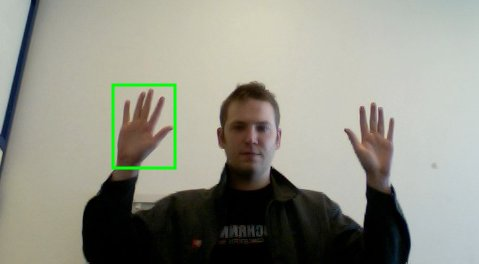
\includegraphics[width=0.45\linewidth]{figures/template/good.jpg}}
\hspace{0.03\linewidth}
\subfloat[result of template search]{\label{fig:template_occlusion}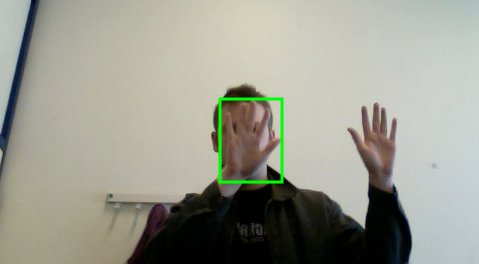
\includegraphics[width=0.45\linewidth]{figures/template/occlusion.jpg}}
\end{center}
\caption{Example of template search}
\label{fig:templatesearch}
\end{figure}

\autoref{fig:templatesearch} shows a test setting of a template search. In the left image The left hand was found using the skin model. In the second frame the hand cannot be found, because it is occluding the face and using the skin model approach the hand will be labeled as face. Using a template search the hand can still be tracked.


\section{Discussion}
This method is quite robust, but can fail if the conditions listed in \autoref{sec:goal} are not met. See \autoref{fig:fail} for an example of failed segmentation. This figure is a still from one of the movies in the dataset used in the experiments. The test subject has a skin color profile that is similar to parts of the background. Not much can be done to solve this problem, except the threshold can be manually adjusted. Still, this will introduce more false negatives and the segmentation will still be poor.

\begin{figure}[htbp]
\center{}
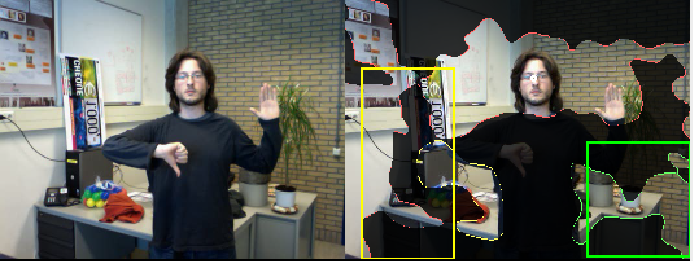
\includegraphics[width=0.8\linewidth]{figures/fail.png}
\caption{Example of failed segmentation}
\label{fig:fail}
\end{figure}

Also, it requires manual tweaking of one parameter - the threshold for going from the probabilistic domain to the binary domain. The adaptive threshold could be used to remove the need for this parameter, but becomes very slow with a high neighborhood value. A high neighborhood value is required, since a low value doesn't perform very well. Also the background is clustered as a big blob, which requires an extra removal step later on. \autoref{fig:thresholdedAdap} shows the example output of a adaptive threshold with a neighborhood of 51.


\begin{figure}[htbp]
\center{}
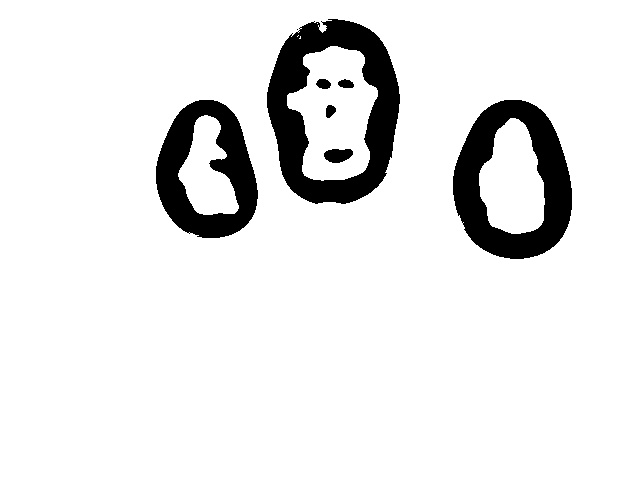
\includegraphics[width=0.3\linewidth]{figures/pipeline/thresholdedAdap.jpg}
\caption{Adaptive threshold with pixel neighborhood of 51}
\label{fig:thresholdedAdap}
\end{figure}






